% !TEX encoding = UTF-8
% !TEX TS-program = pdflatex
% !TEX root = ../nt.tex
% !TEX spellcheck = it-IT

%************************************************
\chapter{Training Facility}
\label{cap:training}
%************************************************\\

\section{Homeworks 1}

\subsection{Esercizio 1}

In fig.1 sono illustrate due topologie di rete per il collegamento tra due sedi di un’azienda. Valutare in quale caso l’affidabilità del collegamento tra le due sedi è maggiore, supponendo che i router IP siano fault-free e che i link di collegamento (una rete fisica di una internetwork IP è considerata un “link” tra due nodi IP) abbiano la stessa affidabilità.

\begin{center}
\begin{figure}[H]
\centering
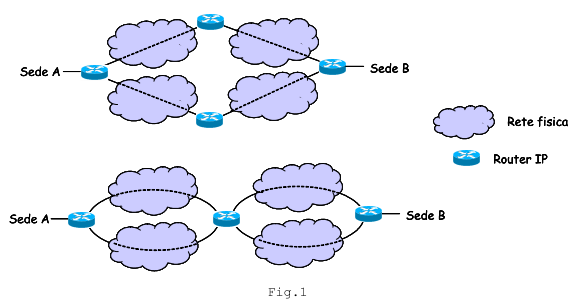
\includegraphics[scale=1]{figures/ex/hw11.png}
\end{figure}
\end{center}

Procediamo naturalmente utilizzando la tecnica degli RBD, date le ipotesi in gioco ed introducendo le opportune ipotesi di indipendenza dei vari link (dei guasti dei vari link in particolare), ponendo $R:=R(t)$:

\begin{itemize}

\item{\textit{parallelo di due SERIE}}: $[R_1=1-(1-R^2)^2]$;
\item{\textit{serie di due PARALLELO}}: $[R_2=[1-(1-R)^2]^2]$;

\end{itemize}


Naturalmente, è di gran lunga migliore l'affidabilità del secondo collegamento (coefficienti maggiori in numero). Il numero di possibili percorsi interrotti è minimizzato, per via della maggiore opportunità di collegamento a fronte di guasti.


\subsection{Esercizio 2}

Si consideri un servizio di rete basato su una batteria di $m$ file server. Il servizio è erogato (UP) fino a che almeno l file server sono funzionanti. Ciascun utente accede al servizio tramite una workstation. La porzione di internetwork mostrata in figura collega la LAN lato utente alla LAN lato server. Supponendo che:

\begin{itemize}

\item l’affidabilità dei router IP e delle due LAN sia molto alta;
\item l’affidabilità di ciascun link di collegamento tra i router sia $R_l(t)$ (una rete fisica di una internetwork IP è considerata un “link” tra due nodi IP);
\item l’affidabilità di ciascun file server sia pari a $R_f(t)$;
\item l’affidabilità di ciascuna workstation sia pari a $R_w(t)$;
\item tutti i malfunzionamenti siano indipendenti l’uno dall’altro

\end{itemize}

si valuti l’affidabilità del sistema tramite il quale un utente accede al servizio.

\begin{center}
\begin{figure}[H]
\centering
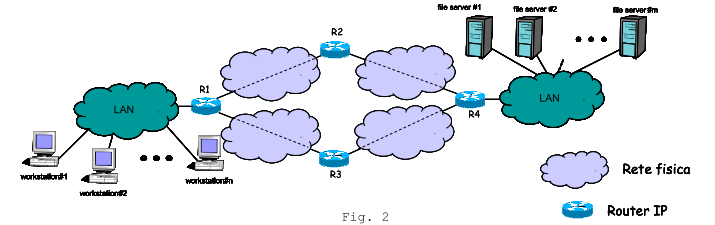
\includegraphics[scale=0.8]{figures/ex/hw12.png}
\end{figure}
\end{center}

Risoluzione: $m$ file server. Servizio UP quando abbiamo $l$ ne sono funzionanti. Blocchi indipendenti e struttura semplice $\implies$ RBD utilizzabile:

\[
	R_w(t)[1-(1-R_l(t))^2]^2\sum_{i=l}^m{\binom{m}{i}R_f(t)^i[1-R_f(t)]^{m-i}}
\]


\subsection{Esercizio 3}

In fig.3 è illustrata la topologia di rete per il collegamento tra le tre sedi di un’azienda. Valutare l’affidabilità del collegamento della sede A con la sede C supponendo che i router IP siano fault-free, che i link di collegamento abbiano la stessa affidabilità e che non vi siano loop per le rotte.           
Fig.3  
Si supponga, adesso, che il link R2-R3 abbia una capacità $C_1\ (bit/sec)$ molto minore della capacità $C_2\ (bit/sec)$ dei rimanenti link e che siano attive due sessioni di comunicazione: una prima sessione S1 i cui pacchetti viaggiano dalla sede A alla sede C lungo la rotta R1-R4-R3, una seconda sessione S2 i cui pacchetti viaggiano dalla sede B alla sede C lungo la rotta R2-R4-R3 (visto che $C_1<<C_2$). Si assuma che i pacchetti associati alla sessione S1 arrivino al router R1 secondo un processo di Poisson a velocità $X_{S1}$, che i pacchetti associati alla sessione S2 arrivino al router R2 secondo un processo di Poisson a velocità $X_{S2}$. Le lunghezze dei pacchetti siano v.c. i.i.d. con distribuzione esponenziale a valor medio $L$ bit. Si supponga, infine, di poter trascurare i ritardi di elaborazione e propagazione e che i buffer dei router abbiano una dimensione molto grande. Si derivi la CMTC omogenea che puo’ essere utilizzata per lo studio della distribuzione del ritardo di pacchetto associato alla sessione S1.

\begin{center}
\begin{figure}[H]
\centering
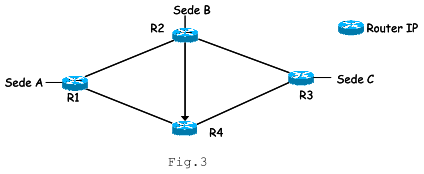
\includegraphics[scale=1]{figures/ex/hw13.png}
\end{figure}
\end{center}

Risoluzione: supponiamo router fault-free e link di collegamento \underline{alla stessa affidabilità}, e \underline{NO LOOP tra le rotte}!

Si valuti l'affidabilità supponendo $L_{2-4}$ HALF-DUPLEX (unidirezionale), e supponendo che NON vi siano LOOP. NO struttura semplice, sebbene siano blocchi indipendenti a valle della riduzione. Applichiamo il \textit{Key-Item Method}, supponendo $L_{4-3}$ come elemento chiave. Alla fine avremo:

\[
	R_S(t) = R_a(t)R_i(t) + R_b(t)(1-R_i(t))
\]

\begin{itemize}

\item

Consideriamo il primo SCENARIO: $L_{4-3}$ cortocircuitato: abbiamo il parallelo di un semplice blocco con la serie di un blocco e del parallelo di due blocchi:

\[
	[R_a(t) := 1-(1-R)(1-R[1-(1-R)^2])]
\]

\item

Nel secondo scenario, $L_{4-3}$ è un circuito aperto. Dato che se si attraversa $L_{1-4}$ non si può risalire per via dell'unidirezionalità di $L_{2-4}$, e d'altro canto se si prende $L_{2-4}$ a valle dell'attraversamento di $L_{1-2}$ non si può comunque risalire sulla sinistra per via dell'ipotesi dell'assenza di LOOP, tale scenario collassa nella serie di due semplici blocchi: $R_b(t) := R^2$.

\end{itemize}

Riassemblando opportunamente troviamo:

\[
	R_S(t) = [1-(1-R)(1-R[1-(1-R)^2])]R + R^2(1-R)
\]


Per quanto riguarda il secondo punto, eseguiamo il seguente mapping tra rotte e velocità di arrivo dei vari flussi:

\[	
	\left\{
	\begin{aligned}
	&X_{S1}-POISSON\\
	&X_{S2}-POISSON
	\end{aligned}
	\right.\mapsto\left\{
	\begin{aligned}
	&R1-R4-R3\\
	&R2-R4-R3
	\end{aligned}
	\right.
\]

Sia $C_1\ll C_2$ la capacità del link R2-R3 $([C_i]=[bit/sec])$. Abbiamo che: $\mathit{L}\sim EXP(L\ bit)$. Si trascurino i ritardi di propagazione ed elaborazione, e si supponga che i buffer dei router abbiano una dimensione molto gramde $(\iff d_1,d_2=+\infty)$. La seguente è la CMTC omogenea per lo studio della distribuzione del ritardo dei paccchetti associati alla sessione $S_1$, con rotta: R1-R4-R3. Sfruttando le EQUAZIONI del TRAFFICO troviamo le velocità di arrivo sui vari link che ci servono, in concomitanza anche alla derivazione del rate di trasmissione:

\[
	\left\{
	\begin{aligned}
	&\lambda_{14}=X_{S1}\\
	&\lambda_{43}=\underline{X_{S1}+X_{S2}}\\
	&\frac{C}{L}=\mu [\frac{bit}{sec\ bit} = \frac{bit}{sec}]
	\end{aligned}
	\right.
\]

Abbiamo la seguente CMTC, con STATI TRANSITORI: \{R1, R4\} e STATO ASSORBENTE \{R3\}, rappresentato dal seguente DTT:

\begin{center}
\begin{tikzpicture}[->, >=stealth', auto, semithick, node distance=3cm]
\tikzstyle{every state}=[fill=white,draw=black,thick,text=black,scale=2]
\node[state]    (R1)                     {$R1$};
\node[state]    (R4)[right of=R1]   {$R4$};
\node[state]    (R3)[right of=R4]   {$R3$};
\path
(R1) edge[bend left]     node{$\mu-\lambda_{14}$}         (R4)
(R4) edge[bend left]     node{$\mu-\lambda_{43}$}         (R3);
\node at ($(R3)+(0,-1.5)$) {ABSORBED};
\end{tikzpicture}
\end{center}

I tassi sono riassunti di seguito:

\[
	\left\{
	\begin{aligned}
	&\mu-\lambda_{14},\ R1-R4\\
	&\mu-\lambda_{43},\ R4-R3
	\end{aligned}
	\right.
\]

\section{Homeworks 2}

\subsection{Esercizio 1}

Un servizio di rete è basato su un sistema ridondante parallelo con due dispositivi. La CMTC illustrata in figura 3 rappresenti il modello di disponibilità del sistema. Valutare il Mean Time To Failure (MTTF) del sistema supponendo che lo stato iniziale della CMTC sia lo stato 2. Valutare, in funzione delle probabilità di regime, il numero medio di “Failure” che si hanno durante una finestra temporale di durata pari a T unità di tempo.

\begin{center}
\begin{figure}[H]
\centering
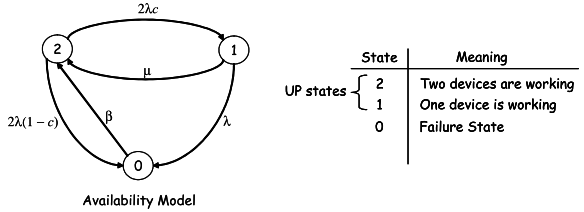
\includegraphics[scale=1]{figures/ex/hw21.png}
\end{figure}
\end{center}

Tale è il DTT:

\begin{center}
\begin{tikzpicture}[->, >=stealth', auto, semithick, node distance=3cm]
\tikzstyle{every state}=[fill=white,draw=black,thick,text=black,scale=1]
\node[state]    (2)                     {$2$};
\node[state]    (1)[right of=2]   {$1$};
\node[state]    (0)[below right of=2]   {$0$};
\path
(2) edge[bend left]     node{$2\lambda c$}         (1)
	edge[bend right,left]     node{$2\lambda (1-c)$}         (0)
(1) edge[bend left]     node{$\lambda$}         (0)
    edge[bend left,below]    node{$\mu$}            (2)
(0) edge   node{$\beta$}             (2);
\end{tikzpicture}
\end{center}

Sistema ridondante parallelo con due dispositivi. $c$ coverage factor, $\lambda=-q_{22}$ velocità totale di uscita dallo stato 2. STARTING STATE = \{2\}. 

\[
	\left\{
	\begin{aligned}
	&T_f\sim EXP(\lambda)\\
	&T_r\sim EXP(\beta)
	\end{aligned}
	\right.
\]

Abbiamo due dispositivi. $\pi_2(0)=1\impliedby$ \{2\} STARTING STATE.

Il modello di disponibilità è quello sintetizzato nel precedente DTT. Per quanto concerne il solo calcolo dell'MTTF, possiamo procedere con la tecnica degli stati assorbenti e dei tempi medi di assorbimento. Consideriamo quindi il relativo modello di calcolo per l'affidabilità: si effettui il detach del ramo di transizione $0\rightarrow 2$. Adesso la CMTC contiene uno stato assorbente: \{0\}:

\begin{center}
\begin{tikzpicture}[->, >=stealth', auto, semithick, node distance=3cm]
\tikzstyle{every state}=[fill=white,draw=black,thick,text=black,scale=1]
\node[state]    (2)                     {$2$};
\node[state]    (1)[right of=2]   {$1$};
\node[state]    (0)[below right of=2]   {$0$};
\path
(2) edge[bend left]     node{$2\lambda c$}         (1)
	edge[bend right,left]     node{$2\lambda (1-c)$}         (0)
(1) edge[bend left]     node{$\lambda$}         (0)
    edge[bend left,below]    node{$\mu$}            (2);
\node at ($(0)+(0,-1)$) {\underline{FAILED}};
\end{tikzpicture}
\end{center}

 Naturalmente la catena in questa configurazione NON è però ERGODICA $\iff\nexists (\pi_i = \lim_{t\to +\infty}{\pi_i(t) = \Pr\{X(t)=i\}})$.

\begin{itemize}

\item{a)} \textbf{MTTF}

Per il primo punto, utilizziamo i risultati dell'esercizio visto precedentemente: \textbf{CMTC with Absorbing States}, e procediamo con la tecnica dei tempi medi di assorbimento. Scriviamo la matrice generatore dei tassi di transizione:

\[
	\bar{Q} =
	\begin{bmatrix}-2\lambda&2\lambda c&2\lambda(1-c)\\ \mu&-(\mu+\lambda)&\lambda\\0&0&0\end{bmatrix} \in\R^{3\times 3}
\]

Adoperiamo ora una restrizione della matrice $\bar{Q}$ considerando solo gli stati transitori, sapendo che $S = N \cup A$:

\[
	\bar{Q}_N =
	\begin{bmatrix}-2\lambda&2\lambda c\\ \mu&-(\mu+\lambda)\end{bmatrix}
\]

Sappiamo che:

\[
	\left\{
	\begin{aligned}
	&L_1(\infty) < +\infty\\
	&L_2(\infty) < +\infty\\
	&L_0(\infty) = +\infty
	\end{aligned}
	\right.
\]

Quindi scriviamo l'equazione matriciale: $\bar{L}_N(\infty)\bar{Q}_N = -\bar{\pi}_N(0)$, avendo cura di alleggerire la notazione: $L_i(\infty) := L_i\ \forall i$:

\[
	\begin{bmatrix}L_2&L_1\end{bmatrix}\begin{bmatrix}-2\lambda&2\lambda c\\ \mu&-(\mu+\lambda)\end{bmatrix} = -\begin{bmatrix}\pi_2(0)&\pi_1(0)\end{bmatrix}
\]

Sapendo che: $\{\pi_2(0)=1,\ \pi_1(0)=\pi_0(0)=0\} \implies$

\[
	\left\{
	\begin{aligned}
	&L_2(-2\lambda)+L_1\mu = -(\pi_2(0)=1)\\
	&L_2(2\lambda c)-L_1(\mu+\lambda) = -(\pi_1(0)=0)
	\end{aligned}
	\right.
\]

Ricordiamo che $[\lim_{t\to +\infty}{L_i(t)} = L_i(\infty)]$. Abbiamo:

\[
	\left\{
	\begin{aligned}
	&L_1 = \frac{-1+2l\lambda L_2}{\mu}\\
	&L_2(2\lambda c) - \frac{(2\lambda L_2 -1)}{\mu}(\mu+\lambda) = 0
	\end{aligned}
	\right. \implies
	\left\{
	\begin{aligned}
	&\left[
	\begin{aligned}
	&2L_2\lambda\mu c - 2\lambda\mu L_2 -2\lambda^2L_2 + \mu + \lambda = 0\\
	&2L_2\lambda(\mu c - \mu-\lambda)+\mu+\lambda = 0\\
	&L_2 = \frac{-(\mu+\lambda)}{2\lambda(\mu c-\mu-\lambda)} = \frac{(\lambda+\mu)}{2\lambda(\mu+\lambda-\lambda c)}
	\end{aligned}
	\right.\\
	&L_1 = \frac{(-1+2\lambda L_2)}{\mu} = \frac{-1+\frac{2\lambda (\lambda+\mu)}{2\lambda(\mu+\lambda-\lambda c)}}{\mu} =\\
	&= \frac{-\mu-\lambda+\lambda c+\lambda+\mu}{(\mu+\lambda-\lambda c)\mu}
	\end{aligned}
	\right.
\]

Quindi abbiamo: 

\[
	MTTA_1+MTTA_2=MTTF_1+MTTF_2=L_1(\infty)+L_2(\infty) := L_2+L_1 =
\]
\[
	= \frac{(\lambda+\mu)}{2\lambda(\mu+\lambda-\mu c)} + \frac{c}{(\mu+\lambda-\mu c)} = \frac{\lambda+\mu+2\lambda c}{2\lambda(\mu+\lambda-\mu c)}
\]

Dimensionalmente torna!

\item{b)} \textbf{Numero medio di "Failure" in finestra temporale} $T$:

Per completare l'esercizio, riprendiamo il modello di calcolo per la disponibilità, ove esiste la distribuzione di regime, e calcoliamo il numero medio di failure che si hanno durante una finestra temporale di durata $T[s]$. Sommiamo le frequenze delle transizioni relative all'evento: "Ingresso nello stato di failure", esprimibile ovviamente in funzione delle probabilità di regime:

\[
	f_F := \pi_2 2\lambda(1-c) + \pi_1\lambda = \lambda[2\pi_2(1-c)+\pi_1]
\]

Moltiplicando per $T$ troviamo effettivamente il numero medio di entrate nello stato di FAILURE durante $T$:

\[
	\bar{N}_F = f_FT = T\lambda[2\pi_2(1-c)+\pi_1]
\]

Anche qui dimensionalmente torna tutto.

\end{itemize}

\subsection{Esercizio 2}

Un Internet Service Provider (ISP) dispone di un sistema per l’accesso remoto degli utenti basato su una batteria di N Remote Access Server (RAS), ciascuno dei quali è dotato di m porte. Il sistema è in grado di riconoscere le richieste di accesso associate ad una classe privilegiata di utenti. Si supponga che tali richieste, ad alta priorità, e che le rimanenti richieste, a bassa priorità, arrivino secondo processi indipendenti di Poisson  a velocità, rispettivamente, $\{\lambda_1,\ \lambda_2\}$. Si assuma, inoltre, che i tempi di collegamento siano v.c. indipendenti e distribuite esponenzialmente con valor medio $\frac{1}{\mu}$. Quando una richiesta ad alta priorità arriva ed una porta qualsiasi sui vari apparati RAS è disponibile (“idle”), la richiesta è accettata e la porta è assegnata ad essa, altrimenti la richiesta è scartata. Una richiesta a bassa priorità è accettata solo se $(g+1)$ o più porte sono disponibili, altrimenti la richiesta è scartata.  I RAS sono soggetti a malfunzionamenti. Il “time to failure” ed il “time to repair” per un RAS siano v.c. indipendenti e distribuite esponenzialmente con parametro, rispettivamente, pari a: $\{f,\ \beta\}$. Una singola “repair facility” sia condivisa da tutti i RAS. Introducendo eventuali ipotesi che si ritengono necessarie, il candidato valuti la probabilità $P_H$ che una richiesta ad alta priorità sia scartata. Suggerimento. Se si trascurano gli effetti che hanno sulla quantità a regime $P_H$ gli eventi corrispondenti al guasto di un RAS quando ci sono collegamenti in corso sulle sue porte, il problema può essere affrontato con un approccio gerarchico.  
Il candidato immagini, adesso, di essere collegato ad Internet tramite l’ISP di cui sopra. Valuti la probabilità $P_I$ che il proprio collegamento sia interrotto improvvisamente a seguito del guasto del RAS.

Risoluzione:

(ISP) Internet Service Provider, con batteria di $N:=\cardinality{RAS}$ (Remote Access Server). Ogni RAS è dotato di $m:=\cardinality{porte}$. Si ha il seguente mapping:

\[
	\left\{
	\begin{aligned}
	&\lambda_1-POISSON\\
	&\lambda_2-POISSON
	\end{aligned}
	\right. \mapsto
	\left\{
	\begin{aligned}
	&HPRIO\ ARRIVALS\\
	&LPRIO\ ARRIVALS
	\end{aligned}
	\right.
\]

I tempi di collegamento (servizio) siano v.c. indipendenti e distribuite esponenzialmente con valor medio $(\frac{1}{\mu})$. Se arriva una HPRIO-req, allora se ci sono porte disponibili è accettata, altrimenti la richiesta viene scartata. Se invece arriva una LPRIO-req, sono necessarie $(g+1)$ porte per accettare la richiesta, altrimenti anch'essa viene scartata. Abbiamo:

\[	
	\left\{
	\begin{aligned}
	&ttf\sim EXP(f)\\
	&ttr\sim EXP(\beta)
	\end{aligned}
	\right.
\]

Si noti che abbiamo una SRF (Single Repair Facility). Definiamo: $P_H=\Pr\{LOSS\}_{HPRIO}$. Si immagini che gli eventi relativi alla dependability (disponibilità ed affidabilità) siano di gran lunga più rari che quelli relativi alle performance (richieste di collegamento), ed accettando inoltre di trascurare gli effetti che hanno sulle quantità a regime $P_H$ gli eventi comprendenti il guasto di un RAS quando vi sono collegamenti in corso sulle sue $m$ porte, allora il sistema può essere analizzato mediante APPROCCIO GERARCHICO. Immaginiamo che i tempi di collegamento siano indipendenti dai tempi di arrivo delle richieste, e che i tempi di guasto siano indipendenti dai tempi di riparazione (ipotesi più che plausibile, ma non scontata). Approccio gerarchico. Sia suddiviso il modello in:

\begin{itemize}
\item{-)} Modello di disponibilità (\textit{Availability Model});
\item{-)} Performance Model
\end{itemize}

Cominciamo con l'analizzare, per l'appunto gerarchicamente, il sistema:

\begin{itemize}

\item{\underline{\textit{Availability Model}}}:

Diamo come definzione di stato del modello di disponibilità la seguente:

$N(t):=\cardinality{RAS\ funzionanti\ in\ t}$. Tale è il DTT del modello di disponibilità (a livello più alto):

\begin{center}
\begin{tikzpicture}[->, >=stealth', auto, semithick, node distance=2cm]
\tikzstyle{every state}=[fill=white,draw=black,thick,text=black,scale=1.2]
\node[state]    (M)                     {$M$};
\node[state]    (MM1)[right of=M]   {$M-1$};
\node[state]    (MM2)[right of=MM1]   {$M-2$};
\node[state] (d) [right of=MM2] {\ldots};
\node[state]    (1)[right of=d]   {$1$};
\node[state]    (0)[right of=1]   {$0$};
\path
(M) edge[bend left]     node{$Mf$}         (MM1)
(MM1) edge[bend left]     node{$(M-1)f$}         (MM2)
    edge[bend left,below]    node{$\beta$}            (M)
(MM2) edge[bend left]     node{$(M-2)f$}           (d)
    edge[bend left,below]    node{$\beta$}             (MM1)
(d) edge[bend left]         node{$2f$}   (1)
	edge[bend left,below]   node{$\beta$}          (MM2)
(1) edge[bend left]       node{$f$}  (0)
	  edge[bend left,below]   node{$\beta$}     (d)
(0)   edge[bend left,below]  node{$\beta$}          (1);
\end{tikzpicture}
\end{center}

Calcoliamo la velocità totale di uscita, supponendo che $N(t)=M-i$. Definiamo le v.a. $\{\xi_{Rt},\eta_{Rt}\}$ rispettivamente tempo di riparazione residuo e tempo di guasto residuo. Ricordiamo che:

\[
	\left\{
	\begin{aligned}
	&\eta_{jRt}\sim EXP(f)\\
	&\eta_{Rt}\sim EXP((M-i)f)
	\end{aligned}
	\right.
\]

Infatti, di RAS funzionanti ve ne sono $M-i$ con guasti indipendenti tra di loro, quindi $\eta_{Rt}\sim EXP(\sum_k^{M-i}{f_k=f} = (M-i)F)$. Calcoliamo $(\phi_{i':=M-i}(t) = \min(\eta_{Rt},\xi_{Rt}))\sim EXP(-q_{i'i'})$:

\[
	F_{\phi_{M-i}}^c(\tau) = \Pr\{\phi_{M-i}(t)>\tau\} = \Pr\{\min(\eta_{Rt},\xi_{Rt}) >\tau\} = \Pr\{\xi_{Rt}>\tau,\ \eta_{Rt}>\tau\} =
\]
\[
	= \Pr\{\xi_{Rt}>\tau\}\Pr\{\eta_{Rt}>\tau\} = \e^{-\beta\tau}\e^{-[(M-i)f\tau]} =
\]
\[
	= \e^{-[\beta+(M-i)f]\tau} \implies q_{i'i'} = -[\beta+(M-i)f]
\]

Calcoliamo ora i tassi di transizione:

\[
	\tau_{i',i'+1} = \frac{q_{i',i'+1}}{-q_{i'i'}} = \Pr\{\xi_{Rt}<\eta_{Rt}\} = \int_0^\infty{\Pr\{\xi_{Rt}<\eta_{Rt}\ |\ \eta_{Rt}=y\}\Pr\{\eta_{Rt}=y\}dy} =
\]
\[
	= \int_0^\infty{(1-\e^{-\beta y})(M-i)f\e^{-(M-i)fy}dy} =
\]
\[
	= \int_0^\infty{(M-i)f\e^{-(M-i)fy}dy}-(M-i)f\int_0^\infty{\e^{-[\beta+(M-i)f]y}dy} =
\]
\[
	= 1-\frac{(M-i)f}{\beta+(M-i)f} = \frac{\beta+(M-i)f-(M-i)f}{\beta+(M-i)f} \implies q_{i',i'+1} = \beta
\]

Analogamente..

\[
	\tau_{i',i'-1} = \frac{q_{i',i'-1}}{-q_{i'i'}} = \Pr\{\eta_{Rt}<\xi_{Rt}\} = \int_0^\infty{\Pr\{\eta_{Rt}<\xi_{Rt}\ |\ \xi_{Rt}=y\}\Pr\{\xi_{Rt}=y\}dy} =
\]
\[
	= \int_0^\infty{(1-\e^{-(M-i)fy})\beta\e^{-\beta y}dy} = \int_0^\infty{\beta\e^{-\beta y}dy}-\beta\int_0^\infty{\e^{-[(M-i)f+\beta]y}dy} =
\]
\[
	= 1-\frac{\beta}{(M-i)f+\beta} = \frac{(M-i)f+\beta-\beta}{(M-i)f+\beta} = \frac{(M-i)f}{(M-i)f+\beta} \implies q_{i',i'-1}=(M-i)f
\]

Per quanto concerne le probabilità a regime abbiamo:

\[
	\left\{
	\begin{aligned}
	&\pi_i=\pi_0(\frac{\beta}{f})^i \frac{1}{i!}\\
	&[\pi_0=\frac{1}{\sum_{i=0}^M{(\frac{\beta}{f})^i \frac{1}{i!}}}
	\end{aligned}
	\right.
\]

con $0\leq i\leq M$. La formula è già stata vista in realtà nella M/M/m/0, ovvero la B di ERLANG.

\item{\underline{\textit{Performance Model}}}:

Una porta per una richiesta a bassa priorità si occupa solo se $(g+1)$ porte sono ancora disponibili. Potremmo considerare come definizione di stato: $Y(t):=\cardinality{porte\ occupate\ in\ t}$, od analogamente: $Y(t):=\cardinality{richieste\ in\ esecuzione\ in\ t}$. Una richiesta verrebbe scartata ovviamente (sia LPRIO che HPRIO) qualora tutte le porte fossero busy, che in tutto sono proprio $mi$ (considerando che vi siano $i$ server funzionanti al tempo $t$). \`E ragionevole ipotizzare che i tassi di transizione (di morte) in questa CMTC, se vi sono $j$ richieste in esecuzione, siano pari proprio a $(j\mu)$, per gli argomenti trattati sempre (minimo di v.a. esponenziali indipendenti). Per scrivere il DTT, ragioniamo sul seguente tableau indicante le richieste rimanenti:

\[
	\left\{
	\begin{aligned}
	&mi\\
	&mi-1\\
	&mi-2\\
	&\vdots\\
	&\left[
	\begin{aligned}
	&mi-k=g+1\\
	&k:=mi-g-1
	\end{aligned}
	\right.
	\end{aligned}
	\right.
\]

Il DTT è allora il seguente:

\begin{center}
\begin{tikzpicture}[->, >=stealth', auto, semithick, node distance=2cm]
\tikzstyle{every state}=[fill=white,draw=black,thick,text=black,scale=1]
\node[state]    (0)                     {$0$};
\node[state]    (1)[right of=0]   {$1$};
\node[state]    (2)[right of=1]   {$2$};
\node[state] (d1) [right of=2] {\ldots};
\node[state]    (mg1)[right of=d1]   {$k+1$};
\node[state]    (d2)[right of=mg1]   {\ldots};
\node[state] 	(mi)[right of=d2]    {$mi$};
\path
(0) edge[bend left]     node{$\lambda$}         (1)
(1) edge[bend left]     node{$\lambda$}         (2)
    edge[bend left,below]    node{$\mu$}            (0)
(2) edge[bend left]     node{$\lambda$}           (d1)
    edge[bend left,below]    node{$2\mu$}             (1)
(d1) edge[bend left]         node{$\lambda$}   (mg1)
	edge[bend left,below]   node{$3\mu$}          (2)
(mg1) edge[bend left]       node{$\lambda_1$}  (d2)
	  edge[bend left,below]   node{$(k+1)\mu$}     (d1)
(d2)  edge[bend left]  node{$\lambda_1$}          (mi)
	  edge[bend left,below]   node{$(k+2)\mu$}     (mg1)
(mi) edge[bend left,below]   node{$mi\mu$}     (d2);
\end{tikzpicture}
\end{center}

Solita storia per i tassi di transizione. Se consideriamo uno stato $j$ prima di $(mi-g-1)$, allora la velocità di arrivo delle richieste, effettuando un POOLING alla POISSON è: $\lambda := \lambda_1+\lambda_2$. Al solito:

\[
	\left\{
	\begin{aligned}
	&\xi_{Rt}\sim EXP(\lambda)\\
	&\eta_{Rt}\sim EXP(j\mu)
	\end{aligned}
	\right.
\]

\[
	(\phi_j(t) = \min(\xi_{Rt},\eta_{Rt}))\sim EXP(-q_{jj}) \implies
\]
\[
	\implies F_{\phi_j}(\tau) = \Pr\{\phi_j(t)>\tau\} = \Pr\{\min(\xi_{Rt},\eta_{Rt})>\tau\} = \Pr\{\xi_{Rt}>\tau,\ \eta_{Rt}>\tau\} =
\]
\[
	= \Pr\{\xi_{Rt}>\tau\}\Pr\{\eta_{Rt}>\tau\} = \e^{-\lambda\tau}\e^{-j\mu\tau}=\e^{-(\lambda+j\mu)\tau} \implies -q_{jj}=(\lambda+j\mu)
\]

Calcoliamo ora i tassi di transizione:

\[
	\tau_{j,j+1}=\frac{q_{j,j+1}}{-q_{jj}} = \Pr\{\xi_{Rt}<\eta_{Rt}\} = \int_0^\infty{\Pr\{\xi_{Rt}<\eta_{Rt}\ |\ \eta_{Rt}=y\}\Pr\{\eta_{Rt}=y\}dy} =
\]
\[
	= \int_0^\infty{(1-\e^{-\lambda y})j\mu\e^{-j\mu y}dy} = \int_0^\infty{j\mu\e^{-j\mu y}dy}-j\mu\int_0^\infty{\e^{-(\lambda+j\mu)}dy} =
\]
\[
	= 1-\frac{j\mu}{\lambda+j\mu}\int_0^\infty{(\lambda+j\mu)\e^{-(\lambda+j\mu)y}dy} = 1-\frac{j\mu}{\lambda+j\mu} =
\]
\[
	= \frac{\lambda+j\mu-j\mu}{\lambda+j\mu} = \frac{\lambda}{\lambda+j\mu} \implies q_{j,j+1}=\lambda
\]

Analogamente:

\[	
	\tau_{j,j-1}=\frac{q_{j,j-1}}{-q_{jj}} = \Pr\{\eta_{Rt}<\xi_{Rt}\} = \int_0^\infty{\Pr\{\eta_{Rt}<\xi_{Rt}\ |\ \xi_{Rt}=y\}\Pr\{\xi_{Rt}=y\}dy} =
\]
\[
	= \int_0^\infty{(1-\e^{-j\mu y})\e^{-\lambda y}dy} = \int_0^\infty{\lambda\e^{-\lambda y}dy}-\lambda\int_0^\infty{\e^{-(\lambda+j\mu)y}dy} =
\]
\[
	= 1-\frac{\lambda}{(\lambda+j\mu)}\int_0^\infty{(\lambda+j\mu)\e^{-(\lambda+j\mu)y}dy} = \frac{\lambda+j\mu-\lambda}{\lambda+j\mu} = \frac{j\mu}{\lambda+j\mu} \implies q_{j,j-1}=j\mu 
\]

Facciamo una sintesi:

\[
	\tau_{j,j+1} = \left\{
	\begin{aligned}
	&\frac{\lambda}{\lambda+j\mu},\ j<mi-g\\
	&\frac{\lambda_1}{\lambda_1+j\mu},\ j\geq mi-g
	\end{aligned}
	\right.
\]

\[
	\left\{
	\begin{aligned}
	&P_j = \left\{
	\begin{aligned}
	&P_0(\frac{\lambda}{\mu})^j \frac{1}{j!},\ j<mi-g\\
	&P_0(\frac{\lambda_1}{\mu})^j \frac{\lambda^{mi-g-1}}{\lambda_1^{mi-g-1}j!},\ j\geq mi-g
	\end{aligned}
	\right.\\
	&P_0 = \frac{1}{1+\sum_{j=1}^{mi-g-1}{(\frac{\lambda}{\mu})^j \frac{1}{j!}} + \frac{\lambda^{mi-g-1}}{\lambda_1^{mi-g-1}}\sum_{j=mi-g}^{mi}{(\frac{\lambda_1}{\mu})^j \frac{1}{j!}}}
	\end{aligned}
	\right.
\]

\end{itemize}

Con la seguente procedura faremo un mapping tra i due modelli:

\[
	\underline{P_L(i)} := P_{mi}^{(a)} \stackrel{PASTA}{=} P_{mi} =
\]
\[
	= \frac{(\frac{\lambda_1}{\mu})^{mi} \frac{\lambda^{mi-g-1}}{\lambda_1^{mi-g-1} (mi)!}}{\sum_{j=0}^{mi-g-1}{(\frac{\lambda}{\mu})^j \frac{1}{j!}} + \frac{\lambda^{mi-g-1}}{\lambda_1^{mi-g-1}}\sum_{j=mi-g}^{mi}{(\frac{\lambda_1}{\mu})^j \frac{1}{j!}}}
\]

ove abbiamo opportunamente inglobato il termine 1 nella prima sommatoria. Effettuiamo il seguente assegnamento:

\[
	\left\{
	\begin{aligned}
	&r_i := P_L(i),\ i=1,2,\ \dots,M\\
	&\left[
	\begin{aligned}
	&\E[z] = \sum_{i=0}^M{r_i\pi_i} = \sum_{i=0}^M{P_L(i)\pi_i} =\\
	&= \sum_{i=1}^M{P_L(i)\pi_i} + (r_0=1)
	\end{aligned}
	\right.
	\end{aligned}
	\right.
\]

Calcoliamo ora la probabilità $P_I$ che il collegamento di un utente su un RAS sia interrotto improvvisamento a seguito del guasto di quest'ultimo. Ridefiniamo opportunamente i tempi residui, indicando rispettivamente con $\{\eta_{Rt},\xi_{Rt}\}$ il tempo di failure residuo ed il tempo di servizio residuo:

\[
	\left\{
	\begin{aligned}
	&\eta_{Rt}\sim EXP(f)\\
	&\xi_{Rt}\sim EXP(\mu)
	\end{aligned}
	\right.
\]

\[
	\Pr\{\eta_{Rt}<\xi_{Rt}\} = \int_0^\infty{\Pr\{\eta_{Rt}<\xi_{Rt}\ |\ \xi_{Rt}=y\}\Pr\{\xi_{Rt}=y\}dy} =
\]
\[
	= \int_0^\infty{(1-\e^{-fy})\mu\e^{-\mu y}dy} = \int_0^\infty{\mu\e^{-\mu y}}-\mu\int_0^\infty{\e^{-(f+\mu)y}dy} =
\]
\[
	= 1-\frac{\mu}{(f+\mu)} = \frac{f+\mu-\mu}{(f+\mu)} = [\frac{f}{f+\mu}]
\]
	

\subsection{Esercizio 3}

Un servizio di rete è erogato tramite un sistema ridondante parallelo costituito da due dispositivi, con un dispositivo active, l’altro in standby. Il failure rate dell’unità attiva è differente da quello dell’unità in standby ed anche gli effetti di un guasto dell’unità attiva sono differenti dagli effetti di un guasto dell’unità in standby. Si supponga che:

\begin{itemize}

\item il time to failure dell’unità attiva sia una v.c. $(\dots)\sim EXP(\lambda)$;
\item il time to failure dell’unità in standby sia una v.c. $(\dots)\sim EXP(\lambda_S)$;
\item il time to restoration di una unità failed sia una v.c. $(\dots)\sim EXP(\mu)$
\end{itemize}
 
Quando l’unità attiva si guasta, con probabilità $c$ (coverage factor) lo switch di protezione ripristina il servizio con successo, commutando sull’unità in standby, la quale diventa l’unità attiva. Con probabilità $(1-c)$, invece, la procedura di ripristino non ha successo ed è necessario un reboot dello switch la cui durata è una v.c. $(\dots)\sim EXP(\beta)$. Un guasto dell’unità in standby mentre l’unità attiva è ancora operativa è rilevato immediatamente con probabilità $c_S$. Con probabilità $(1-c_S)$, invece, il guasto non è rilevato. In tal caso, vi sarebbe un guasto latente dell’unità di riserva. Al fine di rivelare il guasto latente dell’unità in standby, una routine di diagnostica è eseguita ad intervalli di tempo che sono v.c. $(\dots)\sim EXP(\alpha)$.

\begin{itemize}

\item{a)} Definire una CMTC che modelli il sistema e disegnarne il diagramma dei tassi di transizione;
\item{b)} Valutare la frequenza delle riparazioni (supponendo di aver calcolato la distribuzione di regime);
\item{c)} Il servizio non è erogato (sistema DOWN) durante la fase di reboot e quando entrambe le unità sono guaste:

\begin{itemize}

\item Determinare la steady-state unavailability del servizio (supponendo di aver calcolato la distribuzione di regime);
\item Impostare (non risolvere) il sistema di equazioni $\bar{L}_N(\infty)\bar{Q}_N = -\bar{\pi}_N(0)$ (stato iniziale: entrambi i dispositivi non sono guasti) che consente di valutare il Mean Time To Failure del servizio.

\end{itemize}

\end{itemize}

\begin{center}
\begin{figure}[H]
\centering
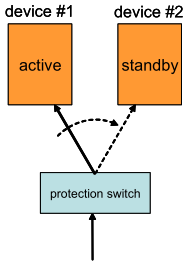
\includegraphics[scale=1]{figures/ex/hw23.png}
\end{figure}
\end{center}

Il DTT è il seguente:

\begin{center}
\begin{tikzpicture}[->, >=stealth', auto, semithick, node distance=3cm]
\tikzstyle{every state}=[fill=white,draw=black,thick,text=black,scale=1]
\node[state]    (2)                     {$2$};
\node[state]    (1)[right of=2]   {$1$};
\node[state]    (0)[right of=1]   {$0$};
\node[state]    (RB)[below right of=2] {$RB$};
\node[state]    (DET)[above of=0] {$DET$}; 
\node[state]    (LAT)[above of=2] {$LAT$};
\path
(2) edge[bend left,below]     node{$\lambda c$}         (1)
    edge[bend right,left]    node{$\lambda (1-c)$}     (RB)
    edge    node{$\lambda_S c_S$}     (DET)
    edge[bend left,left]    node{$\lambda_S(1-c_S)$}     (LAT)
(1) edge[bend left]     node{$\lambda$}         (0)
    edge[bend left]    node{$\mu$}              (2)
    edge[bend left,below]    node{$\mu$}            (2)
(0) edge[bend left,below]    node{$(2)\mu$}             (1)
(LAT)edge[bend left] node{$\alpha$}   (DET)
(DET)edge [bend right,above]   node{$\mu$}         (2)
     edge   node{$\lambda$}     (0)
(RB)edge[right] node{$\beta$}   (1);
\node at ($(0)+(0,-0.8)$) {FAILED};
\end{tikzpicture}
\end{center}

Previo mapping delle seguenti variabili:

\[
	\left\{
	\begin{aligned}
	&\xi_{1Rt}\sim EXP(\lambda)\\
	&\xi_{2Rt}\sim EXP(\lambda_S)
	\end{aligned}
	\right.
\]

$\rightarrow$ \{tempo di guasto residuo al tempo $t$ (ACTIVE), tempo di guasto residuo al tempo $t$ (STANDBY)\}, calcoliamo la velocità totale di uscita dallo STARTING STATE: \{2\}, sapendo che ovviamente $(\phi_2(t)=\min(\xi_{1Rt},\ \xi_{2Rt}))\sim EXP(-q_{22})$:

\[
	F_{\phi_2}(\tau) = \Pr\{\min(\xi_{1Rt},\ \xi_{2Rt})>\tau\} = \Pr\{\xi_{1Rt}>\tau,\ \xi_{2Rt}>\tau\} =
\]
\[
	= \Pr\{\xi_{1Rt}>\tau\}\Pr\{\xi_{2Rt}>\tau\} = \e^{-\lambda\tau}\e^{-\lambda_S\tau} = \e^{-(\lambda+\lambda_S)\tau}
\]

Ciò ovviamente implica che $\implies -q_{22}=\lambda+\lambda_S$.

\underline{Sappiamo empiricamente che}:

\[
	\left\{
	\begin{aligned}
	&q_{21}=c\lambda\\
	&q_{2RB}=(1-c)\lambda\\
	&q_{2DET} = c_S\lambda_S\\
	&q_{2LAT} = (1-c_S)\lambda_S
	\end{aligned}
	\right.
\]

Valutiamo le frequenze delle riparazioni (supponendo ovviamente di aver calcolato la distribuzione di regime). Anzitutto, la CMTC è OMOGENEA (tassi di transizione costanti), \underline{irriducibile} (tutti gli stati comunicano tra di loro) con un numero di stati finito $(\iff \cardinality{stati}<+\infty) \implies$ ERGODICA $\iff \underline{\exists \pi_i=\lim_{t\to +\infty}{\pi_i(t)}}$. Quindi per sapere la frequenza delle riparazioni è sufficiente sommare le frequenze delle transizioni di stato che caratterizzano una riparazione:

\[
	f_R := \pi_1\mu + \pi_0\mu + \pi_{DET}\mu = \mu(\pi_1+\pi_0+\pi_{DET})
\]

Servizio NON EROGATO: (sistema DOWN) durante la fase di reboot e quando entrambe le unità sono guaste. Sempre supponendo di disporre della distribuzione di regime, abiamo che la \textit{STEADY-STATE UNAVAILABILITY} è:

\[
	SSU := \underline{\bar{A} = \pi_0+\pi_{RB}}
\]

Si noti che il tasso $0\rightarrow 1$ dipende dal fatto se abbiamo una SRF (Single Repair Facility) o meno (minimo di v.a. esponenziali indipendenti $\rightarrow$ ancora esponenziale con parametro somma dei ttr dei due dispositivi). Comunque non ci interessa, dal momento che per calcolare l'MTTF del sistema dobbiamo switchare sul modello di affidabilità, che non prevede assolutamente riparazioni. Siamo quindi obbligati a fare il detach del ramo di transizione sopracitato. Per quanto concerne $RB\rightarrow 1$, probabilmente non è considerato poi un guasto catastrofico, un failure molto dannoso dal punto di vista dell'affidabilità; quindi un'attenta analisi dei requisiti potrebbe risparmiarne la cancellazione nel RCM (\textit{Reliability Computational Model}). Impostiamo il sistema: $\bar{L}_N(\infty)\bar{Q}_N = -\bar{\pi}_N(0)$, con stato iniziale: $\{2\} \iff \pi_2(0)=1$. Scriviamo la matrice generatore della catena, ovvero la matrice dei tassi di transizione:

\[
	\bar{Q} = \begin{bmatrix}-(\lambda+\lambda_S)&\lambda c&0&\lambda(1-c)&\lambda_S(1-c_S)&\lambda_S c_S\\ \mu&-(\mu+\lambda)&\lambda&0&0&0\\0&0&0&0&0&0\\0&\beta&0&-\beta&0&0\\0&0&0&0&-\alpha&\alpha\\ \mu&0&\lambda&0&0&-\mu\end{bmatrix}
\]

Si noti che nella CMTC non abbiamo considerato un eventuale ramo di transizione $LAT\rightarrow 0$. Infatti, se la routine di diagnostica fosse eseguita sul primo server, un eventuale guasto di quest'ultimo abbatterebbe il relativo processo di diagnostica in corso, rendendo di fatto impossibile la rilevazione del malfunzionamento del server standby che avesse avuto un malfunzionamento. Ma consideriamo $\alpha\ll \lambda$, in maniera tale che sia molto meno probabile che accada. Comunque è solamente questione di non appesantire il modello. Naturalmente in un'analisi più dettagliata tali questioni andrebbero tenute in conto, magari con l'aggiunta di un watch-dog a parte con il quale effettuare diagnostica e controllo.

Adoperiamo la restrizione della matrice sul set degli stati transitori, ricordando l'ovvia relazione di unione: $S = N\cup A$:

\[
	\left\{
	\begin{aligned}
	\bar{Q}_N &= \begin{bmatrix}-(\lambda+\lambda_S)&\lambda c&\lambda(1-c)&\lambda_S(1-c_S)&\lambda_S c_S\\ \mu&-(\mu+\lambda)&0&0&0\\0&\beta&-\beta&0&0\\0&0&0&-\alpha&\alpha\\ \mu&0&0&0&-\mu\end{bmatrix}\\
	\bar{L}_N &=\begin{bmatrix}L_2&L_1&L_{RB}&L_{LAT}&L_{DET}\end{bmatrix}\\
	\bar{\pi}_N &=\begin{bmatrix}1&0&0&0&0\end{bmatrix}
	\end{aligned}
	\right.
\]

$\bar{L}_N(\infty)\bar{Q}_N = -\bar{\pi}_N(0) \implies$

\[	
	\left\{
	\begin{aligned}
	&-L_2(\lambda+\lambda_S)+L_1\mu+L_{DET}\mu = -1\\
	&L_2\lambda c -L_1(\mu+\lambda) + L_{RB}\beta = 0\\
	&L_2\lambda(1-c)-L_{RB}\beta = 0\\
	&L_2\lambda_S(1-c_S)-L_{LAT}\alpha = 0\\
	&L_2\lambda_S c_S + L_{LAT}\alpha - L_{DET}\mu = 0
	\end{aligned}
	\right.
\]

\section{MTTF of a fiber link}


Transmission links can be deployed with protection channels, wherein if the primary link is disrupted, the system switches to a protection channel. Fiber cable is typically the transmission medium of choice for these link systems. Figures 1, 2 and 3 show the structure of link systems. Link systems can be generally classified as one of three cases: 

\begin{itemize}

\item{\textit{\textbf{Case A}: Unprotected link}} is the single-fiber system with no backup (shown in Fig. 1);
\item{\textit{\textbf{Case B}: Partially protected link}} has redundant fiber media backup. Redundant circuits are supposed to take different physical paths (shown in Fig. 2);
\item{\textit{\textbf{Case C}: Fully protected link}} has fiber media, transceiver, and power backup, with the transceivers being  in  hot standby (shown in Fig. 3).                          

\end{itemize}

\begin{center}
\begin{figure}[H]
\centering
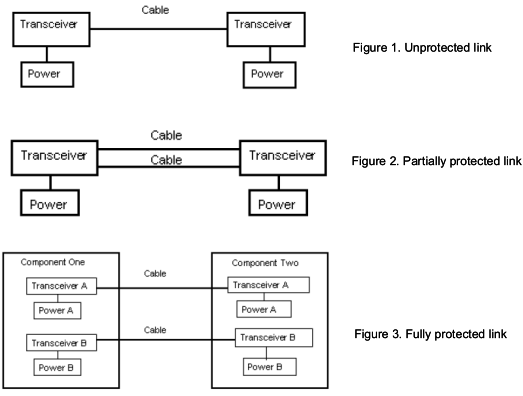
\includegraphics[scale=0.8]{figures/ex/mttffl.png}
\caption{Unprotected link, Partially protected link, Fully protected link}
\end{figure}
\end{center}

For long optical fiber links, cable cuts are the dominant failure scenario (table 1 
shows the optical fiber MTTF at different distances). Instead, for short fiber links (less than about 5 miles), the optical fiber MTTF is quite high, so that the transceiver and power systems become the dominant contribution to failure, rather than the fibers. Assuming that the Transceiver MTTF is equal to $8.0\ years$, that the Power MTTF is equal to $8.0\ years$ and that the Times To Failure of a fiber cable, a power supply and a transceiver are independent, exponentially distributed random variables, evaluate:

\begin{itemize}

\item{a)} the MTTF of a $10-mile$ link without protection;
\item{b)} the MTTF of a $10-mile$, partially protected link;
\item{c)} the MTTF of a $10-mile$ link, fully protected link.
\end{itemize}

\begin{figure}[H]
\centering
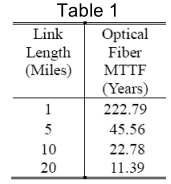
\includegraphics[scale=1]{figures/ex/mttfflt.png}
\end{figure}

Risoluzione:

\[
	\left\{
	\begin{aligned}
	&ttf_{FIBER\_CAB}\sim EXP(h_F=\frac{1}{MTTF_F=22.78y})\\
	&ttf_{TRANS}\sim EXP(h_T=\frac{1}{MTTF_T=8.0y})\\
	&ttf_{POWER}\sim EXP(h_P=\frac{1}{MTTF_P=8.0y})
	\end{aligned}
	\right.
\]

ove $h_i$ sono failure rate. In particolare, la distribuzione del lifetime $(ttf)_i$ è esponenziale $\implies$ failure rate costante e pari a $(\lambda_i:=h_i(t))$. Il valor medio è $\frac{1}{h_i(t)}=(\frac{1}{\lambda_i})$.

\begin{itemize}

\item{\textbf{Unprotected link}}:

In tal primo caso abbiamo la serie di tre macrocomponenti in serie, costituiti rispettivamente da:

\begin{itemize}

\item serie tra power e transceiver a monte;
\item link di trasmissione;
\item serie tra transceiver e power a valle;
\end{itemize}

Nelle configurazioni serie i failure rate si sommano per dar luogo al failure rate complessivo del sistema:

\[
	h_L = 2h_P+2h_t+h_F = (\frac{1}{22.78}y^{-1})+2(\frac{1}{8}y^{-1})+2(\frac{1}{8}y^{-1}) =
\]
\[
	= (\frac{1}{22.78}y^{-1} + \frac{1}{2}y^{-1}) = 0.5439y^-1 \implies \underline{MTTF_L} = \frac{1}{h_L} = \frac{1}{0.5439}y = 1.8386y
\]

\item{\textbf{Partially protected link}}:

In tal caso la configurazione rimane la medesima del caso precedente, ma nell'intermezzo come sistema di trasmissione abbiamo il parallelo tra due link in fibra ottica. Calcoliamo prima l'affidabilità:

\[
	R(t) = R_P(t)^2R_T(t)^2[1-(1-R_F(t))^2] = \e^{-2h_Pt}\e^{-2h_Tt}[-\e^{-2h_Ft}+2\e^{-h_Ft}] =
\]
\[
	= -\e^{-[2h_P+2h_T+2h_F]t}+2\e^{-[2h_P+2h_T+h_F]t}
\]

Quindi integrando opportunamente l'affidabilità, troviamo l'MTTF:

\[
	MTTF = \E[X] = \int_0^\infty{R(t)dt} = 2\int_0^\infty{\e^{-[2h_P+2h_T+h_F]t}dt}-\int_0^\infty{\e^{-[2h_P+2h_T+2h_F]t}dt} =
\]
\[
	= \frac{2}{2h_P+2h_T+h_F}-\frac{1}{2h_P+2h_T+2h_F} = \frac{2}{2(\frac{1}{8})+2(\frac{1}{8})+\frac{1}{22.78}}-\frac{1}{\frac{1}{2}+\frac{2}{22.78}} = 1.976y
\]

Ragionevolmente maggiore!

\item{\textbf{Fully protected link}}:

Dobbiamo fare il parallelo tra i due interi sistemi, ove ogni singolo sistema è quello del caso 1, ovvero l'unprotected link, che ha come affidabilità banalmente:

\[
	R_{NP} = R_P^2 R_T^2 R_F = \e^{-[2h_P+2hT+h_F]t}
\]

Dunque, adoperando il parallelo su $R_{NP}$, doppiandolo opportunamente, abbiamo:

\[
	1-(1-R_{NP})^2 = 1-(1+\e^{-2[2h_P+2h_T+h_F]t} -2\e^{-[2h_P+2h_T+h_F]t}) =
\]
\[
	= 2\e^{-[2h_P+2h_T+h_F]t} - \e^{-2[2h_P+2h_T+h_F]t}
\]

Integrando opportunamente per trovare l'MTTF troviamo:

\[
	MTTF = \E[X] = \int_0^\infty{R(t)dt} = 2\int_0^\infty{\e^{-[2h_P+2h_T+h_F]t}dt} - \int_0^\infty{\e^{-2[2h_P+2h_T+h_F]t}} =
\]
\[
	= \frac{2}{2h_P+2h_T+h_F}-\frac{1}{2[2h_P+2h_T+h_F]} =
\]
\[
	= \frac{3}{2[2h_P+2h_T+h_F]} = \frac{3}{2(0.5439y^{-1})} = 2.75787y
\]

Decisamente migliore!

\end{itemize}


\section{Response Time Distribution 2}

Un servizio di rete è basato su due centri di servizio. In figura 1 è riportata 
la rete di Jackson che descrive lo schema secondo il quale i job sono eseguiti. 
La $P\{accodamento\}$ sia pari, rispettivamente, a $P_A$ per il sistema a coda “A” e a 
$P_B$  per il sistema a coda “B”. Si derivi la CMTC che consente di determinare 
un’approssimazione della distribuzione del tempo di esecuzione di un job.

\begin{center}
\begin{figure}[H]
\centering
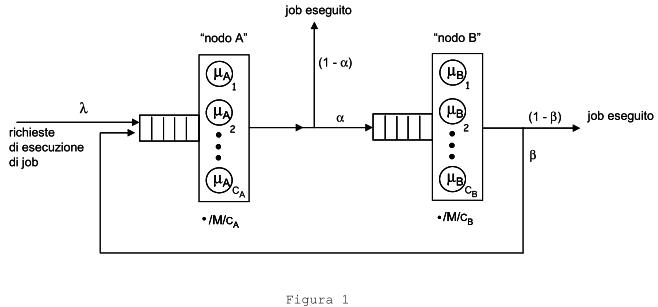
\includegraphics[scale=0.8]{figures/ex/rtd2.png}
\end{figure}
\end{center}

Sia: $P_A:=\Pr\{queueing\}_A,\ P_B:=\Pr\{queueing\}_B$. Dallo studio fatto sappiamo che sono calcolabili mediante C di ERLANG per delle M/M/m. Valgano le ipotesi standard BCMP, dal momento che ci troviamo dinanzi delle code $\mathord{\cdot}$/M/$c_{i\in{A,B}}$, ovvero con arrivi non markoviani (poissoniani). Per A abbiamo:

\[
	T_A = \frac{1}{\mu_A} + P_A \frac{1}{C_A\mu_A(1-\rho_A)} = \frac{C_A(1-\rho_A)+P_A}{\mu_A C_A(1-\rho_A)}
\]

Di conseguenza il tasso di ritardo per questa CMTC, con STATO ASSORBENTE \{OUT\} è:

\[
	q_{AB} = \frac{1}{T_A} = [\frac{C_A(1-\rho_A)+P_A}{\mu_A C_A(1-\rho_A)}]\alpha
\]

Analogamente per l'altro sistema a coda. Quindi i tassi alla fine saranno i seguenti:

\[
	\left\{
	\begin{aligned}
	&q_{AB} = \frac{1}{T_A}\alpha = [\frac{C_A(1-\rho_A)+P_A}{\mu_A C_A(1-\rho_A)}]\alpha\\
	&q_{AOUT} = \frac{1}{T_A}(1-\alpha) = [\frac{C_A(1-\rho_A)+P_A}{\mu_A C_A(1-\rho_A)}](1-\alpha)\\
	&q_{BA} = \frac{1}{T_B}\beta = [\frac{C_B(1-\rho_B)+P_B}{\mu_B C_B(1-\rho_B)}]\beta\\
	&q_{BOUT} = \frac{1}{T_B}(1-\beta) = [\frac{C_B(1-\rho_B)+P_B}{\mu_B C_B(1-\rho_B)}](1-\beta)
	\end{aligned}
	\right.
\]

Il DTT della CMTC è il seguente:

\begin{center}
\begin{tikzpicture}[->, >=stealth', auto, semithick, node distance=3cm]
\tikzstyle{every state}=[fill=white,draw=black,thick,text=black,scale=2]
\node[state]    (CA)                     {$C_A$};
\node[state]    (CB)[right of=CA]   {$C_B$};
\node[state]    (OUT)[below of=CB]   {$OUT$};
\path
(CA) edge[bend left]     node{$[\frac{C_A(1-\rho_A)+P_A}{\mu_A C_A(1-\rho_A)}]\alpha$}         (CB)
     edge[bend right,left]    node{$[\frac{C_A(1-\rho_A)+P_A}{\mu_A C_A(1-\rho_A)}](1-\alpha)$} (OUT)
(CB) edge[bend left]     node{$[\frac{C_B(1-\rho_B)+P_B}{\mu_B C_B(1-\rho_B)}]\beta$}         (CA)
     edge[bend left,right]     node{$[\frac{C_B(1-\rho_B)+P_B}{\mu_B C_B(1-\rho_B)}](1-\beta)$} (OUT);
\node at ($(OUT)+(0,-1.5)$) {ABSORBED};
\end{tikzpicture}
\end{center}


\section{Server Load Balancer}

Un Server Load Balancer (SLB) (vedi figura) è utilizzato da un Content Service 
Provider per bilanciare il carico sui k server di una server farm. L’algoritmo 
adottato dal SLB per distribuire le richieste di servizio dei client è il 
seguente: una nuova richiesta viene inoltrata al server che sta rispondendo al 
minor numero di richieste e, nel caso in cui più server stiano rispondendo allo 
stesso ed, al contempo, più basso numero di richieste, la richiesta è inoltrata 
ad uno qualsiasi tra questi server. 
Si supponga: 

\begin{itemize}

\item{a)} che le richieste di servizio arrivino al SLB secondo un processo 
indipendente di Poisson a velocità $\lambda\ [req/s]$; 
\item{b)} che sia trascurabile l’intervallo temporale tra l’istante in cui una 
richiesta arriva al SLB e l’istante in cui il server selezionato riceve 
tale richiesta; 
\item{c)} che i server rispondano ad una richiesta non appena la ricevono e con 
tempi di servizio che sono variabili casuali indipendenti e distribuite 
esponenzialmente a valor medio $\frac{1}{\mu}$ secondi; 
\item{d)} che un generico server non possa rispondere contemporaneamente a più di $M$ 
richieste e che sia persa qualsiasi richiesta in arrivo quando la server 
farm è satura (ciascun server sta rispondendo a M richieste).

\end{itemize}

Nel caso in cui $k=M=2$,

\begin{itemize}
\item{1)} Disegnare il diagramma dei tassi di transizione di una CMTC che modella il 
sistema e discutere l’ergodicità della catena; 
\item{2)} Calcolare: 

\begin{itemize} 
\item la probabilità che una richiesta di servizio non sia persa; 
\item il numero medio di richieste a cui un server risponde 
contemporaneamente; 
\end{itemize}

\item{3)} La sequenza delle richieste ricevute da un server possono essere modellate 
con un processo di Poisson? Motivare la risposta.

\end{itemize}

\begin{center}
\begin{figure}[H]
\centering
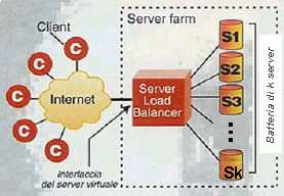
\includegraphics[scale=1]{figures/ex/slb.png}
\caption{Service Load Balancer}
\end{figure}
\end{center}

Risoluzione:

(SLB) as \textit{Service Load Balancer}, (ISP) as \textit{Content Service Provider}. $k$ server di una server farm. Consideriamo la seguente definizione di stato: $N(t):=\cardinality{richieste\ al\ tempo\ t}$. Abbiamo la seguente CMTC, con $[k=M=2]$, rappresentata mediante il seguente DTT:

\begin{center}
\begin{tikzpicture}[->, >=stealth', auto, semithick, node distance=3cm]
\tikzstyle{every state}=[fill=white,draw=black,thick,text=black,scale=1]
\node[state]    (0)                     {$0$};
\node[state]    (1)[right of=0]   {$1$};
\node[state]    (2)[right of=1]   {$2$};
\node[state]    (3)[right of=2]   {$3$};
\node[state]    (4)[right of=3]   {$4$};
\path
(0) edge[bend left]     node{$\lambda$}         (1)
(1) edge[bend left]     node{$\lambda$}         (2)
    edge[bend left]     node{$\mu$}         (0)
(2) edge[bend left]     node{$\lambda$}         (3)
    edge[bend left]     node{$2\mu$}         (1)
(3) edge[bend left]     node{$\lambda$}         (4)
    edge[bend left]     node{$3\mu$}         (2)
(4)edge[bend left]     node{$4\mu$}         (3);
\end{tikzpicture}
\end{center}

La quale è OMOGENEA, IRRIDUCIBILE e con numero di stati finito $(\iff \cardinality{stati}<+\infty)$, dunque è ERGODICA. Probabilità che una richiesta di servizio in arrivo non sia persa:

\[
	P_{NOT4} := 1-\pi_4^{(a)} \stackrel{PASTA}{=} 1-\pi_4 =
\]
\[
	= 1-[\Pr\{N(t)=4\} = \frac{(\frac{\lambda}{\mu})^4 \frac{1}{4!}}{\sum_{i=0}^4{(\frac{\lambda}{\mu})^4 \frac{1}{4!}}}]
\]

Calcoliamo ora il numero medio di richieste a cui un server risponde 
contemporaneamente, ovvero il numero medio di clienti in un server sostanzialmente. Dal momento che i server sono praticamente identici, equifunzionali ed equiprobabili, non c'è nessuna ragione per la quale un arrivo, a parità di richieste sui singoli server, debba preferibilmente esser preso in considerazione dall'uno o dall'altro. In taluna circostanza infatti, l'algoritmo adopera una scelta casuale. Quindi la velocità di arrivo ad ognuno di essi è: $(\frac{\lambda_S}{2})$, sebbene queste velocità NON costituiscano un processo di POISSON, dal momento che vi sono perdite in gioco. Dobbiamo sostanzialmente sommare tutte le frequenze di transizione che riguardano l'ingresso di una richiesta ad uno qualsiasi dei due server:

\[
	\left\{
	\begin{aligned}
	&\lambda_S = \pi_1\mu + \pi_2(2\mu) + \pi_3(3\mu) + \pi_4(4\mu)\\
	&\lambda_S = \lambda\pi_0 + \lambda\pi_1 + \lambda\pi_3 + \lambda\pi_4
	\end{aligned}
	\right.
\]

Ove le due equazioni del sistema sono per l'appunto equivalenti, dal momento che valgono le equazioni di \textit{BILANCIAMENTO LOCALE} per catene di nascita e morte: $\lambda\sum_{i=0}^{k+M-1}{\pi_i} = \underline{\lambda(1-\pi_4)}$. Dopodiché, dal momento che arrivano metà richieste ad uno e metà all'altro, abbiamo che la velocità di arrivo al singolo server è $(\frac{\lambda_S}{2})$, ovvero il relativo throughput per server. Applicando Little banalmente troviamo:

\[
	\bar{N}_S = \frac{\lambda_S}{2}(\frac{1}{\mu})
\]

ove $(\frac{1}{\mu})$ è il tempo medio di permanenza di una richiesta all'interno del singolo server. In linea generale, per un tal modello che rispecchi il sistema reale del genere, vale la seguente equazione:

\[
	\bar{N}_S = \frac{[\lambda_S = \lambda(1-\pi_M)]}{k} (\frac{1}{\mu}) 
\]